%\VignetteEngine{knitr::knitr}
%\VignetteIndexEntry{Flexible Logo plots of symbols and alphanumeric strings using Logolas}
%\VignettePackage{Logolas}

% To compile this document
% library('knitr'); rm(list=ls()); knit('Logolas/vignettes/logolas.Rnw')
% library('knitr'); rm(list=ls()); knit2pdf('Logolas/vignettes/logolas.Rnw'); openPDF('logolas.pdf')
% !Rnw weave = knitr

\documentclass[12pt]{article}\usepackage[]{graphicx}\usepackage[usenames,dvipsnames]{color}
%% maxwidth is the original width if it is less than linewidth
%% otherwise use linewidth (to make sure the graphics do not exceed the margin)
\makeatletter
\def\maxwidth{ %
  \ifdim\Gin@nat@width>\linewidth
    \linewidth
  \else
    \Gin@nat@width
  \fi
}
\makeatother

\definecolor{fgcolor}{rgb}{0.345, 0.345, 0.345}
\newcommand{\hlnum}[1]{\textcolor[rgb]{0.686,0.059,0.569}{#1}}%
\newcommand{\hlstr}[1]{\textcolor[rgb]{0.192,0.494,0.8}{#1}}%
\newcommand{\hlcom}[1]{\textcolor[rgb]{0.678,0.584,0.686}{\textit{#1}}}%
\newcommand{\hlopt}[1]{\textcolor[rgb]{0,0,0}{#1}}%
\newcommand{\hlstd}[1]{\textcolor[rgb]{0.345,0.345,0.345}{#1}}%
\newcommand{\hlkwa}[1]{\textcolor[rgb]{0.161,0.373,0.58}{\textbf{#1}}}%
\newcommand{\hlkwb}[1]{\textcolor[rgb]{0.69,0.353,0.396}{#1}}%
\newcommand{\hlkwc}[1]{\textcolor[rgb]{0.333,0.667,0.333}{#1}}%
\newcommand{\hlkwd}[1]{\textcolor[rgb]{0.737,0.353,0.396}{\textbf{#1}}}%
\let\hlipl\hlkwb

\usepackage{framed}
\makeatletter
\newenvironment{kframe}{%
 \def\at@end@of@kframe{}%
 \ifinner\ifhmode%
  \def\at@end@of@kframe{\end{minipage}}%
  \begin{minipage}{\columnwidth}%
 \fi\fi%
 \def\FrameCommand##1{\hskip\@totalleftmargin \hskip-\fboxsep
 \colorbox{shadecolor}{##1}\hskip-\fboxsep
     % There is no \\@totalrightmargin, so:
     \hskip-\linewidth \hskip-\@totalleftmargin \hskip\columnwidth}%
 \MakeFramed {\advance\hsize-\width
   \@totalleftmargin\z@ \linewidth\hsize
   \@setminipage}}%
 {\par\unskip\endMakeFramed%
 \at@end@of@kframe}
\makeatother

\definecolor{shadecolor}{rgb}{.97, .97, .97}
\definecolor{messagecolor}{rgb}{0, 0, 0}
\definecolor{warningcolor}{rgb}{1, 0, 1}
\definecolor{errorcolor}{rgb}{1, 0, 0}
\newenvironment{knitrout}{}{} % an empty environment to be redefined in TeX

\usepackage{alltt}

\newcommand{\Logolas}{\textit{Logolas}}
\usepackage{dsfont}
\usepackage{cite}



\RequirePackage{/Library/Frameworks/R.framework/Versions/3.3/Resources/library/BiocStyle/resources/tex/Bioconductor}

\AtBeginDocument{\bibliographystyle{/Library/Frameworks/R.framework/Versions/3.3/Resources/library/BiocStyle/resources/tex/unsrturl}}



\author{Kushal K Dey \\[1em]
\small{\textit{Stephens Lab}, Dept. of Statistics, The University of Chicago} \mbox{ }\\
\small{\texttt{$^*$Correspondending Email: kkdey@uchicago.edu}}}


\bioctitle[ Flexible Logo plots of symbols and alphanumeric strings using \Logolas{}]{Flexible Logo plots of symbols and alphanumeric strings using \Logolas{}}
\IfFileExists{upquote.sty}{\usepackage{upquote}}{}
\begin{document}

\maketitle

\begin{abstract}
\vspace{1em}
Logo plots are popular in genomic studies for sequence alignment and motif detection. However, logo plots have been restrictive in its scope due to limited size of the library of symbols used by logo plotting tools and packages  and the lack of flexibility in extending it to other applications. In this package, we provide an easy and flexible interface for the user to plot logos. More importantly, we extend the library of logos from A, C, T, G (library of symbols in seqLogo) and English alphabets (library of symbols in RWebLogo, motifStack) to include numbers and alpha-numeric strings with provision for punctuations and arrows. It also provides the user with a simple graphical interface to create her own logo and add to her personal library.
In this vignette, we discuss a number of applications in genomics and beyond where such flexible logo plots can be effective in visualizing patterns.

\vspace{1em}
\textbf{\Logolas{} version:} 0.99.8 \footnote{This document used the vignette from \Bioconductor{} package \Biocpkg{CountClust, DESeq2} as \CRANpkg{knitr} template}
\end{abstract}



\newpage

\tableofcontents

\section{Introduction}

Logo plots are a popular tool in bioinformatics and regulatory genomics studies for representing sequence alignment patterns and for sequence and protein motif detection. One of the first and widely used logo plotting tools is \Biocpkg{seqLogo} by Oliver Bembom \cite{Bembom2016}, specifically targeted at DNA sequence alignment. However, it has a library of only 4 symbols - A, C, G and T- corresponding to the 4 nucleotides. The package \CRANpkg{RWebLogo} is an extension of WebLogo python package that plots custom sequence logos by extending it to all alphabets \cite{Wagih2014}. Another package \Biocpkg{motifStack} works with both DNA/RNA sequence motif and amino acid sequence motif and customizes font size and colors \cite{Ou2015}.

\Logolas{} adds more flexibility by customizing logos and the graphical design of the logo plots. Also it extends the library of symbols beyond English alphabets to numbers, symbols (arrows, punctuations) and to alphanumeric strings. It allows the user to choose a range of information criteria to determine logo sizes. It provides a simple user interface to create new logos and add them to their personalized library of logos and even apply them in strings. We show several applications in genomics, ecology and document mining, where such logo plots can be applied.

\newpage

\section{\Logolas{} Installation}

\Logolas{} requires the following CRAN-R package : \CRANpkg{grid}, \CRANpkg{gridExtra}, \CRANpkg{RColorBrewer}, \CRANpkg{devtools}.

\begin{knitrout}
\definecolor{shadecolor}{rgb}{0.969, 0.969, 0.969}\color{fgcolor}\begin{kframe}
\begin{alltt}
\hlkwd{source}\hlstd{(}\hlstr{"http://bioconductor.org/biocLite.R"}\hlstd{)}
\hlkwd{biocLite}\hlstd{(}\hlstr{"Logolas"}\hlstd{)}
\end{alltt}
\end{kframe}
\end{knitrout}

For the developmental version on Github, one can use

\begin{knitrout}
\definecolor{shadecolor}{rgb}{0.969, 0.969, 0.969}\color{fgcolor}\begin{kframe}
\begin{alltt}
\hlstd{devtools}\hlopt{::}\hlkwd{install_github}\hlstd{(}\hlstr{'kkdey/Logolas'}\hlstd{)}
\end{alltt}
\end{kframe}
\end{knitrout}

Then load the package with:

\begin{knitrout}
\definecolor{shadecolor}{rgb}{0.969, 0.969, 0.969}\color{fgcolor}\begin{kframe}
\begin{alltt}
\hlkwd{library}\hlstd{(Logolas)}
\end{alltt}
\end{kframe}
\end{knitrout}

\section{Applications}

We start with the most basic application of logo plots - for alignment of DNA sequence, comprising of logos A, C, T and G, corresponding to the four nucleotide. This is the typical application of \Biocpkg{seqLogo}. We start with the same demo example provided in the \Biocpkg{seqLogo} vignette.

\begin{figure}[h]
\begin{center}
\begin{knitrout}
\definecolor{shadecolor}{rgb}{0.969, 0.969, 0.969}\color{fgcolor}\begin{kframe}
\begin{alltt}
\hlstd{mFile} \hlkwb{<-} \hlkwd{system.file}\hlstd{(}\hlstr{"Exfiles/pwm1"}\hlstd{,} \hlkwc{package}\hlstd{=}\hlstr{"seqLogo"}\hlstd{)}
\hlstd{m} \hlkwb{<-} \hlkwd{read.table}\hlstd{(mFile)}
\hlstd{p} \hlkwb{<-} \hlstd{seqLogo}\hlopt{::}\hlkwd{makePWM}\hlstd{(m)}
\hlstd{seqLogo}\hlopt{::}\hlkwd{seqLogo}\hlstd{(p)}
\end{alltt}
\end{kframe}
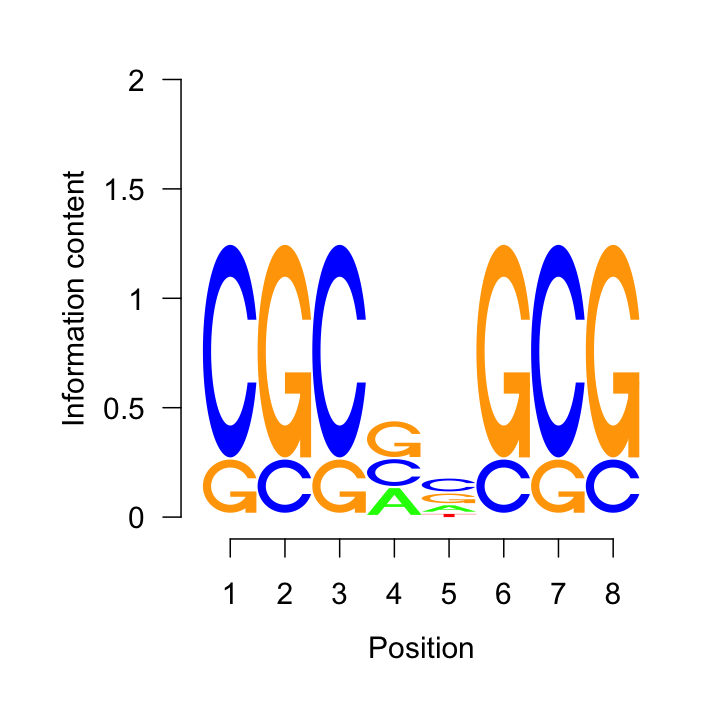
\includegraphics[width=5in,height=5in]{figure/seqlogo_use-1} 

\end{knitrout}
\end{center}
\end{figure}


The user first needs to make a position weight matrix from the matrix using the \begin{verb} makePWM() \end{verb} function. Then it uses the \begin{verb} seqLogo() \end{verb} function on the output to plot the logo plots.

\newpage

Now we apply \Logolas{} to build a similar plot.The user can directly use the `p@pwm` object generated by \begin{verb} seqLogo() \end{verb} as shown below

\begin{knitrout}
\definecolor{shadecolor}{rgb}{0.969, 0.969, 0.969}\color{fgcolor}\begin{kframe}
\begin{alltt}
\hlstd{color_profile} \hlkwb{<-} \hlkwd{list}\hlstd{(}\hlstr{"type"} \hlstd{=} \hlstr{"per_row"}\hlstd{,}
                      \hlstr{"col"} \hlstd{= RColorBrewer}\hlopt{::}\hlkwd{brewer.pal}\hlstd{(}\hlkwd{dim}\hlstd{(p}\hlopt{@}\hlkwc{pwm}\hlstd{)[}\hlnum{1}\hlstd{],}\hlkwc{name} \hlstd{=}\hlstr{"Spectral"}\hlstd{))}
\hlkwd{logomaker}\hlstd{(p}\hlopt{@}\hlkwc{pwm}\hlstd{,}
          \hlkwc{color_profile} \hlstd{= color_profile,}
          \hlkwc{frame_width} \hlstd{=} \hlnum{1}\hlstd{,}
          \hlkwc{ic.scale} \hlstd{=} \hlnum{TRUE}\hlstd{,}
          \hlkwc{yscale_change}\hlstd{=}\hlnum{FALSE}\hlstd{,}
          \hlkwc{xlab}\hlstd{=}\hlstr{"position"}\hlstd{,}
          \hlkwc{col_line_split} \hlstd{=} \hlstr{"grey80"}\hlstd{)}
\end{alltt}
\end{kframe}
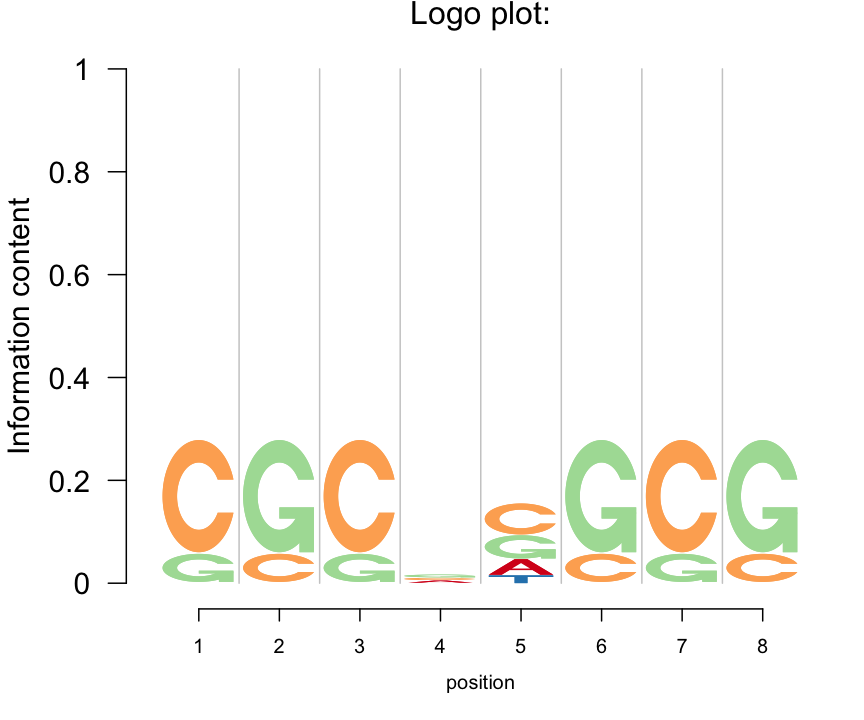
\includegraphics[width=6in,height=5in]{figure/logolas_use_0-1} 

\end{knitrout}

Besides using the `makePWM` format of \begin{verb} seqLogo() \end{verb} package, the user has the flexibility to directly input a matrix with row names and column names as well.

\begin{figure}[h]
\begin{center}
\begin{knitrout}
\definecolor{shadecolor}{rgb}{0.969, 0.969, 0.969}\color{fgcolor}\begin{kframe}
\begin{alltt}
\hlkwd{rownames}\hlstd{(m)} \hlkwb{<-} \hlkwd{c}\hlstd{(}\hlstr{"A"}\hlstd{,} \hlstr{"C"}\hlstd{,} \hlstr{"G"}\hlstd{,} \hlstr{"T"}\hlstd{)}
\hlkwd{colnames}\hlstd{(m)} \hlkwb{<-} \hlnum{1}\hlopt{:}\hlnum{8}
\hlkwd{logomaker}\hlstd{(m,}
          \hlkwc{color_profile} \hlstd{= color_profile,}
          \hlkwc{frame_width} \hlstd{=} \hlnum{1}\hlstd{,}
          \hlkwc{ic.scale} \hlstd{=} \hlnum{TRUE}\hlstd{,}
          \hlkwc{yscale_change}\hlstd{=}\hlnum{FALSE}\hlstd{,}
          \hlkwc{xlab}\hlstd{=}\hlstr{"position"}\hlstd{,}
          \hlkwc{col_line_split} \hlstd{=} \hlstr{"grey80"}\hlstd{)}
\end{alltt}
\end{kframe}
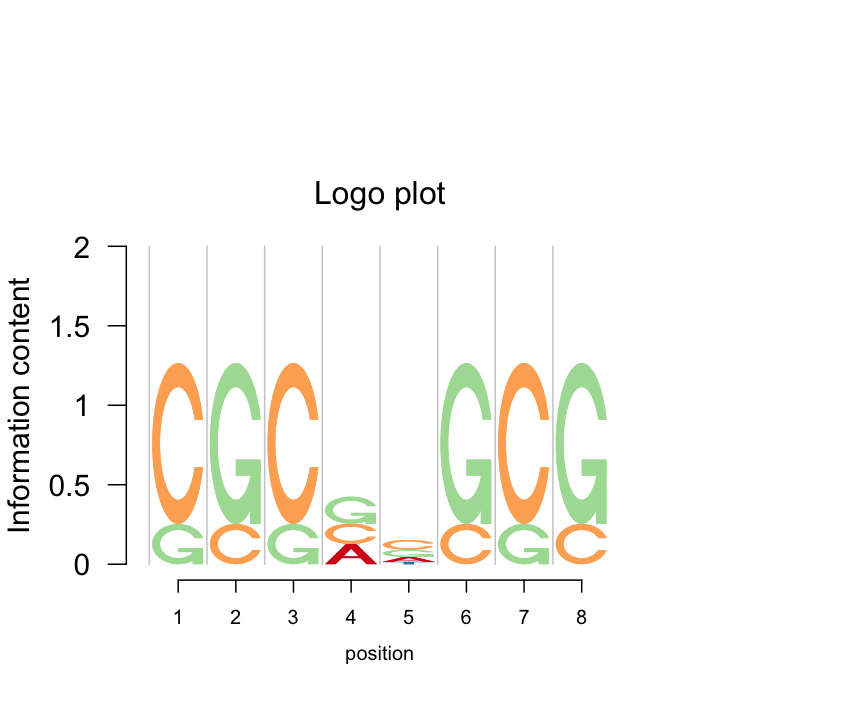
\includegraphics[width=6in,height=5in]{figure/logolas_use-1} 

\end{knitrout}
\end{center}
\end{figure}

\newpage

As default, if \begin{verb} ic.scale = TRUE \end{verb}, the heights of the bars at each position are determined by the Shannon entropy as in \Biocpkg{seqLogo}. The size of logo in each stack is proportional to the relative abundance of that logo in that stack.

To change to other orders of Renyi entropy, one can tune the input parameter \begin{verb} alpha \end{verb}. A higher value of  \begin{verb} alpha \end{verb} makes the logos more prominent, besides maintaining relative structure. One can set different infromation criteria using the \begin{verb} ic_computer \end{verb}
function.

\begin{knitrout}
\definecolor{shadecolor}{rgb}{0.969, 0.969, 0.969}\color{fgcolor}\begin{kframe}
\begin{alltt}
\hlkwd{ic_computer}\hlstd{(m,} \hlkwc{alpha}\hlstd{=}\hlnum{3}\hlstd{)}
\end{alltt}
\begin{verbatim}
## [1] 1.673 1.673 1.673 0.931 0.849 1.673 1.673 1.673
\end{verbatim}
\end{kframe}
\end{knitrout}

Also, the Y-axis can be adjusted by taking \begin{verb} yscale_change=TRUE \end{verb}

\begin{figure}[h]
\begin{center}
\begin{knitrout}
\definecolor{shadecolor}{rgb}{0.969, 0.969, 0.969}\color{fgcolor}\begin{kframe}
\begin{alltt}
\hlkwd{rownames}\hlstd{(m)} \hlkwb{<-} \hlkwd{c}\hlstd{(}\hlstr{"A"}\hlstd{,} \hlstr{"C"}\hlstd{,} \hlstr{"G"}\hlstd{,} \hlstr{"T"}\hlstd{)}
\hlkwd{colnames}\hlstd{(m)} \hlkwb{<-} \hlnum{1}\hlopt{:}\hlnum{8}
\hlkwd{logomaker}\hlstd{(m,}
          \hlkwc{color_profile} \hlstd{= color_profile,}
          \hlkwc{frame_width} \hlstd{=} \hlnum{1}\hlstd{,}
          \hlkwc{ic.scale} \hlstd{=} \hlnum{TRUE}\hlstd{,}
          \hlkwc{alpha} \hlstd{=} \hlnum{2}\hlstd{,}
          \hlkwc{yscale_change}\hlstd{=}\hlnum{TRUE}\hlstd{,}
          \hlkwc{xlab}\hlstd{=}\hlstr{"position"}\hlstd{,}
          \hlkwc{col_line_split} \hlstd{=} \hlstr{"grey80"}\hlstd{)}
\end{alltt}
\end{kframe}
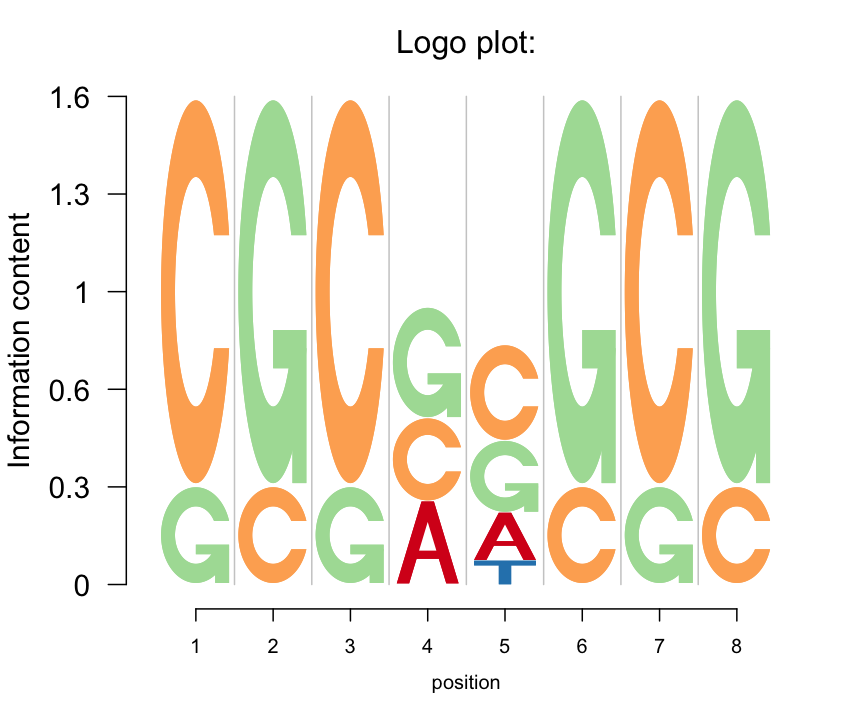
\includegraphics[width=6in,height=5in]{figure/logolas_use_2-1} 

\end{knitrout}
\end{center}
\end{figure}


\newpage

One can also normalize the  heights of the stacks of logos for each column by choosing \begin{verb} ic.scale = FALSE \end{verb}.

\begin{figure}[h]
\begin{center}
\begin{knitrout}
\definecolor{shadecolor}{rgb}{0.969, 0.969, 0.969}\color{fgcolor}\begin{kframe}
\begin{alltt}
\hlkwd{rownames}\hlstd{(m)} \hlkwb{<-} \hlkwd{c}\hlstd{(}\hlstr{"A"}\hlstd{,} \hlstr{"C"}\hlstd{,} \hlstr{"G"}\hlstd{,} \hlstr{"T"}\hlstd{)}
\hlkwd{colnames}\hlstd{(m)} \hlkwb{<-} \hlnum{1}\hlopt{:}\hlnum{8}
\hlkwd{logomaker}\hlstd{(m,}
          \hlkwc{color_profile} \hlstd{= color_profile,}
          \hlkwc{frame_width} \hlstd{=} \hlnum{1}\hlstd{,}
          \hlkwc{ic.scale} \hlstd{=} \hlnum{FALSE}\hlstd{,}
          \hlkwc{alpha} \hlstd{=} \hlnum{2}\hlstd{,}
          \hlkwc{xlab}\hlstd{=}\hlstr{"position"}\hlstd{,}
          \hlkwc{col_line_split} \hlstd{=} \hlstr{"grey80"}\hlstd{,}
          \hlkwc{ylab} \hlstd{=} \hlstr{"Probability"}\hlstd{)}
\end{alltt}
\end{kframe}
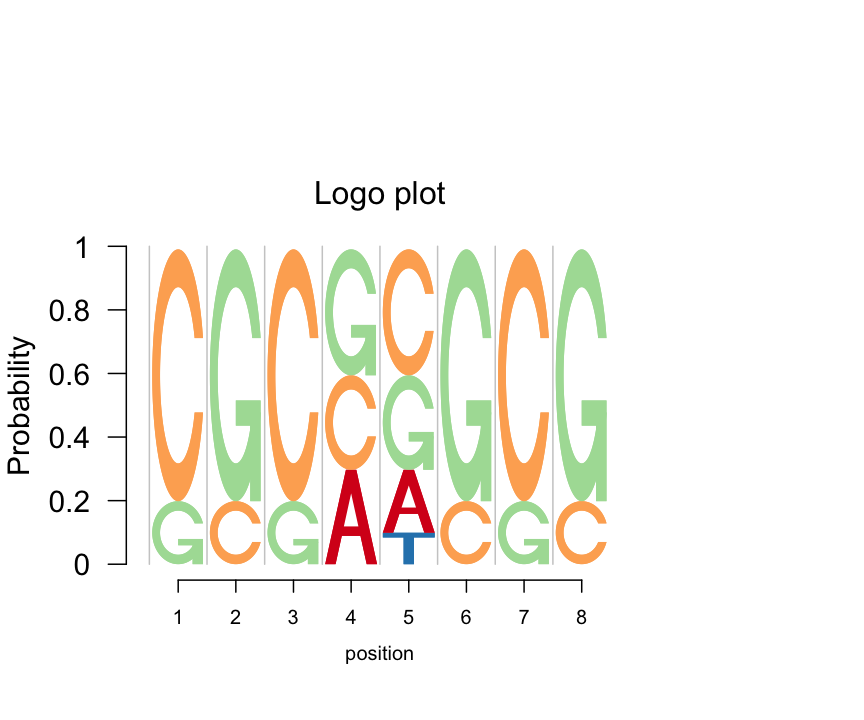
\includegraphics[width=6in,height=5in]{figure/logolas_use_3-1} 

\end{knitrout}
\end{center}
\end{figure}

\newpage

\Logolas{} lets you customize the colors of the logos using \begin{verb} color_profile \end{verb}, has option for user-defined information function under option \begin{verb} ic \end{verb},  beyond the different Renyi criteria that can be set. User can set titles, X-labels, Y-labels, axis ticks and also the relative width of each column of the logo stack, making it much more flexible than the standard packages for logo plotting.

\subsection{Amino acid sequence motif}

One can use \Logolas{} for amino acid sequence motif detection as well, as the logo library of the software includes all the English alphabets and the 20 amino acids have a 1-letter representation using English alphabets.


\begin{knitrout}
\definecolor{shadecolor}{rgb}{0.969, 0.969, 0.969}\color{fgcolor}\begin{kframe}
\begin{alltt}
\hlstd{counts_mat} \hlkwb{<-} \hlkwd{rbind}\hlstd{(}\hlkwd{c}\hlstd{(}\hlnum{0}\hlstd{,} \hlnum{0}\hlstd{,} \hlnum{100}\hlstd{,} \hlnum{1}\hlstd{,} \hlnum{2}\hlstd{),} \hlkwd{c}\hlstd{(}\hlnum{4}\hlstd{,} \hlnum{3}\hlstd{,} \hlnum{30}\hlstd{,} \hlnum{35}\hlstd{,} \hlnum{2}\hlstd{),}
                    \hlkwd{c}\hlstd{(}\hlnum{100}\hlstd{,} \hlnum{0}\hlstd{,} \hlnum{10}\hlstd{,} \hlnum{2}\hlstd{,} \hlnum{7}\hlstd{),}\hlkwd{rep}\hlstd{(}\hlnum{0}\hlstd{,}\hlnum{5}\hlstd{),}
                    \hlkwd{c}\hlstd{(}\hlnum{4}\hlstd{,} \hlnum{2}\hlstd{,} \hlnum{3}\hlstd{,} \hlnum{7}\hlstd{,} \hlnum{70}\hlstd{),} \hlkwd{c}\hlstd{(}\hlnum{1}\hlstd{,} \hlnum{8}\hlstd{,} \hlnum{0}\hlstd{,} \hlnum{60}\hlstd{,} \hlnum{3}\hlstd{),}
                    \hlkwd{rep}\hlstd{(}\hlnum{0}\hlstd{,} \hlnum{5}\hlstd{),} \hlkwd{c}\hlstd{(}\hlnum{4}\hlstd{,} \hlnum{2}\hlstd{,} \hlnum{100}\hlstd{,} \hlnum{1}\hlstd{,} \hlnum{1}\hlstd{),}
                    \hlkwd{c}\hlstd{(}\hlnum{12}\hlstd{,} \hlnum{8}\hlstd{,} \hlnum{16}\hlstd{,} \hlnum{7}\hlstd{,} \hlnum{20}\hlstd{),} \hlkwd{c}\hlstd{(}\hlnum{55}\hlstd{,} \hlnum{0}\hlstd{,} \hlnum{1}\hlstd{,} \hlnum{0}\hlstd{,} \hlnum{12}\hlstd{),}
                    \hlkwd{rep}\hlstd{(}\hlnum{0}\hlstd{,}\hlnum{5}\hlstd{),} \hlkwd{c}\hlstd{(}\hlkwd{rep}\hlstd{(}\hlnum{0}\hlstd{,}\hlnum{3}\hlstd{),} \hlnum{20}\hlstd{,} \hlnum{0}\hlstd{),}
                    \hlkwd{rep}\hlstd{(}\hlnum{0}\hlstd{,}\hlnum{5}\hlstd{),} \hlkwd{c}\hlstd{(}\hlnum{0}\hlstd{,} \hlnum{0}\hlstd{,} \hlnum{30}\hlstd{,} \hlnum{0}\hlstd{,} \hlnum{22}\hlstd{),}
                    \hlkwd{c}\hlstd{(}\hlnum{1}\hlstd{,} \hlnum{0}\hlstd{,} \hlnum{12}\hlstd{,} \hlnum{3}\hlstd{,} \hlnum{10}\hlstd{),} \hlkwd{rep}\hlstd{(}\hlnum{0}\hlstd{,}\hlnum{5}\hlstd{),}
                    \hlkwd{c}\hlstd{(}\hlnum{0}\hlstd{,} \hlnum{1}\hlstd{,} \hlnum{0}\hlstd{,} \hlnum{34}\hlstd{,} \hlnum{1}\hlstd{),} \hlkwd{c}\hlstd{(}\hlnum{0}\hlstd{,} \hlnum{1}\hlstd{,} \hlnum{12}\hlstd{,} \hlnum{35}\hlstd{,} \hlnum{1}\hlstd{),}
                    \hlkwd{c}\hlstd{(}\hlnum{0}\hlstd{,} \hlnum{30}\hlstd{,} \hlnum{1}\hlstd{,} \hlnum{10}\hlstd{,} \hlnum{2}\hlstd{),} \hlkwd{c}\hlstd{(}\hlnum{0}\hlstd{,} \hlnum{1}\hlstd{,} \hlnum{4}\hlstd{,} \hlnum{100}\hlstd{,} \hlnum{2}\hlstd{))}
\end{alltt}
\end{kframe}
\end{knitrout}


\begin{figure}[htp]
\begin{center}
\begin{knitrout}
\definecolor{shadecolor}{rgb}{0.969, 0.969, 0.969}\color{fgcolor}\begin{kframe}
\begin{alltt}
\hlkwd{rownames}\hlstd{(counts_mat)} \hlkwb{<-} \hlkwd{c}\hlstd{(}\hlstr{"A"}\hlstd{,} \hlstr{"R"}\hlstd{,} \hlstr{"N"}\hlstd{,} \hlstr{"D"}\hlstd{,}\hlstr{"C"}\hlstd{,} \hlstr{"E"}\hlstd{,} \hlstr{"Q"}\hlstd{,} \hlstr{"G"}\hlstd{,}
                          \hlstr{"H"}\hlstd{,} \hlstr{"I"}\hlstd{,} \hlstr{"L"}\hlstd{,} \hlstr{"K"}\hlstd{,} \hlstr{"M"}\hlstd{,} \hlstr{"F"}\hlstd{,} \hlstr{"P"}\hlstd{,} \hlstr{"S"}\hlstd{,}
                          \hlstr{"T"}\hlstd{,} \hlstr{"W"}\hlstd{,} \hlstr{"Y"}\hlstd{,} \hlstr{"V"}\hlstd{)}

\hlkwd{colnames}\hlstd{(counts_mat)} \hlkwb{<-} \hlkwd{c}\hlstd{(}\hlstr{"Pos 1"}\hlstd{,} \hlstr{"Pos 2"}\hlstd{,} \hlstr{"Pos 3"}\hlstd{,} \hlstr{"Pos 4"}\hlstd{,} \hlstr{"Pos 5"}\hlstd{)}

\hlstd{cols1} \hlkwb{<-} \hlkwd{c}\hlstd{(}\hlkwd{rev}\hlstd{(RColorBrewer}\hlopt{::}\hlkwd{brewer.pal}\hlstd{(}\hlnum{12}\hlstd{,} \hlstr{"Paired"}\hlstd{))[}\hlkwd{c}\hlstd{(}\hlnum{3}\hlstd{,}\hlnum{4}\hlstd{,}\hlnum{7}\hlstd{,}\hlnum{8}\hlstd{,}\hlnum{11}\hlstd{,}\hlnum{12}\hlstd{,}\hlnum{5}\hlstd{,}\hlnum{6}\hlstd{,}\hlnum{9}\hlstd{,}\hlnum{10}\hlstd{)],}
           \hlstd{RColorBrewer}\hlopt{::}\hlkwd{brewer.pal}\hlstd{(}\hlnum{12}\hlstd{,} \hlstr{"Set3"}\hlstd{)[}\hlkwd{c}\hlstd{(}\hlnum{1}\hlstd{,}\hlnum{2}\hlstd{,}\hlnum{5}\hlstd{,}\hlnum{8}\hlstd{,}\hlnum{9}\hlstd{)],}
           \hlstd{RColorBrewer}\hlopt{::}\hlkwd{brewer.pal}\hlstd{(}\hlnum{9}\hlstd{,} \hlstr{"Set1"}\hlstd{)[}\hlkwd{c}\hlstd{(}\hlnum{9}\hlstd{,}\hlnum{7}\hlstd{)],}
           \hlstd{RColorBrewer}\hlopt{::}\hlkwd{brewer.pal}\hlstd{(}\hlnum{8}\hlstd{,} \hlstr{"Dark2"}\hlstd{)[}\hlkwd{c}\hlstd{(}\hlnum{3}\hlstd{,}\hlnum{4}\hlstd{,}\hlnum{8}\hlstd{)])}

\hlstd{color_profile} \hlkwb{<-} \hlkwd{list}\hlstd{(}\hlstr{"type"} \hlstd{=} \hlstr{"per_row"}\hlstd{,}
                      \hlstr{"col"} \hlstd{= cols1)}

\hlkwd{logomaker}\hlstd{(counts_mat,}
          \hlkwc{color_profile} \hlstd{= color_profile,}
          \hlkwc{frame_width} \hlstd{=} \hlnum{1}\hlstd{,}
          \hlkwc{ic.scale}  \hlstd{=} \hlnum{FALSE}\hlstd{,}
          \hlkwc{yscale_change} \hlstd{=} \hlnum{FALSE}\hlstd{)}
\end{alltt}
\end{kframe}
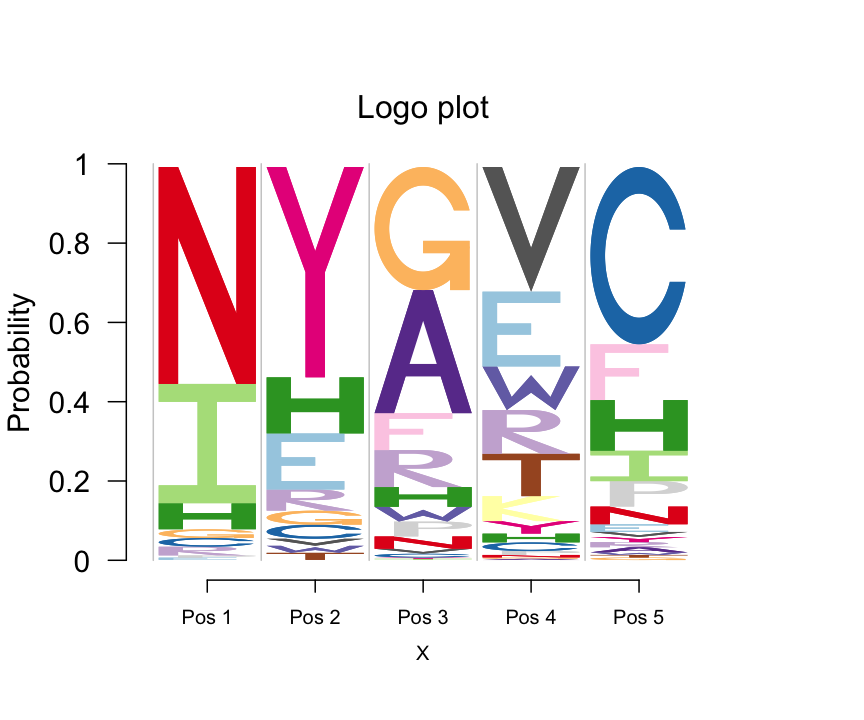
\includegraphics[width=6in,height=5in]{figure/logolas_use_5-1} 

\end{knitrout}
\end{center}
\end{figure}

Note that all one needs to do to build the logo plots is to specify the row names and column names as per the the logos and the stack labels and then fix the colors for the logos.

\newpage

\subsection{String Logos: Mutation profiling}

We now step beyond alphabet logos and present the first example of how a string can be used as a logo. Suppose for a set of cell lines, we are provided data on the number of mutations (nucleotide substitions) and nucleotides at the flanking bases of the nucleotide substitution. This is the kind of problem addressed by Shiraishi et al 2015 \cite{Shiraishi2015}. They developed a package \begin{verb} pmsignature \end{verb} for plotting the substitution and flanking bases profile, but here we use logos to do the same. We apply it here on a demo example.

\begin{knitrout}
\definecolor{shadecolor}{rgb}{0.969, 0.969, 0.969}\color{fgcolor}\begin{kframe}
\begin{alltt}
\hlstd{mFile} \hlkwb{<-} \hlkwd{system.file}\hlstd{(}\hlstr{"Exfiles/pwm1"}\hlstd{,} \hlkwc{package}\hlstd{=}\hlstr{"seqLogo"}\hlstd{)}
\hlstd{m} \hlkwb{<-} \hlkwd{read.table}\hlstd{(mFile)}
\hlstd{p} \hlkwb{<-} \hlstd{seqLogo}\hlopt{::}\hlkwd{makePWM}\hlstd{(m)}
\hlstd{pwm_mat} \hlkwb{<-} \hlkwd{slot}\hlstd{(p,}\hlkwc{name} \hlstd{=} \hlstr{"pwm"}\hlstd{)}
\hlstd{mat1} \hlkwb{<-} \hlkwd{cbind}\hlstd{(pwm_mat[,}\hlkwd{c}\hlstd{(}\hlnum{3}\hlstd{,}\hlnum{4}\hlstd{)],} \hlkwd{rep}\hlstd{(}\hlnum{0}\hlstd{,}\hlnum{4}\hlstd{), pwm_mat[,}\hlkwd{c}\hlstd{(}\hlnum{5}\hlstd{,}\hlnum{6}\hlstd{)]);}
\hlkwd{colnames}\hlstd{(mat1)} \hlkwb{<-} \hlkwd{c}\hlstd{(}\hlstr{"-2"}\hlstd{,} \hlstr{"-1"}\hlstd{,} \hlstr{"0"}\hlstd{,} \hlstr{"1"}\hlstd{,} \hlstr{"2"}\hlstd{)}
\hlstd{mat2} \hlkwb{<-} \hlkwd{cbind}\hlstd{(}\hlkwd{rep}\hlstd{(}\hlnum{0}\hlstd{,}\hlnum{6}\hlstd{),} \hlkwd{rep}\hlstd{(}\hlnum{0}\hlstd{,}\hlnum{6}\hlstd{),}
              \hlkwd{c}\hlstd{(}\hlnum{0.5}\hlstd{,} \hlnum{0.2}\hlstd{,} \hlnum{0.2}\hlstd{,} \hlnum{0.05}\hlstd{,} \hlnum{0.05}\hlstd{,} \hlnum{0}\hlstd{),}
              \hlkwd{rep}\hlstd{(}\hlnum{0}\hlstd{,}\hlnum{6}\hlstd{),} \hlkwd{rep}\hlstd{(}\hlnum{0}\hlstd{,}\hlnum{6}\hlstd{))}
\hlkwd{rownames}\hlstd{(mat2)} \hlkwb{<-} \hlkwd{c}\hlstd{(}\hlstr{"C>T"}\hlstd{,} \hlstr{"C>A"}\hlstd{,} \hlstr{"C>G"}\hlstd{,}
                    \hlstr{"T>A"}\hlstd{,} \hlstr{"T>C"}\hlstd{,} \hlstr{"T>G"}\hlstd{)}

\hlstd{table} \hlkwb{<-} \hlkwd{rbind}\hlstd{(mat1, mat2)}
\end{alltt}
\end{kframe}
\end{knitrout}

Note that we use the symbols \begin{verb} X>Y \end{verb} to denote the  $X \rightarrow Y$ substitutions. The data contains proportion of logos in each position -  $-2$ left flanking, $-1$ left flanking, mutation, $1$ right flanking and $2$ right flanking. Note that \begin{verb} X>Y \end{verb} type symbols occur only in the middle stack (column) as that is the mutation stack, while the nucleotides $A$, $C$, $T$ and $G$ occur only in the left two and right two flanking bases stacks (columns).

Then we apply \begin{verb} logomaker \end{verb} on that matrix.

\begin{figure}[htp]
\begin{center}
\begin{knitrout}
\definecolor{shadecolor}{rgb}{0.969, 0.969, 0.969}\color{fgcolor}\begin{kframe}
\begin{alltt}
\hlstd{color_profile} \hlkwb{<-} \hlkwd{list}\hlstd{(}\hlstr{"type"} \hlstd{=} \hlstr{"per_row"}\hlstd{,}
                      \hlstr{"col"} \hlstd{= RColorBrewer}\hlopt{::}\hlkwd{brewer.pal}\hlstd{(}\hlkwd{dim}\hlstd{(table)[}\hlnum{1}\hlstd{],}\hlkwc{name} \hlstd{=}\hlstr{"Spectral"}\hlstd{))}

\hlkwd{logomaker}\hlstd{(table,}
          \hlkwc{color_profile} \hlstd{= color_profile,}
          \hlkwc{frame_width} \hlstd{=} \hlnum{1}\hlstd{,}
          \hlkwc{ic.scale} \hlstd{=} \hlnum{TRUE}\hlstd{,}
          \hlkwc{yscale_change}\hlstd{=}\hlnum{TRUE}\hlstd{,}
          \hlkwc{xlab} \hlstd{=} \hlstr{"Position"}\hlstd{,}
          \hlkwc{ylab} \hlstd{=} \hlstr{"Information content"}\hlstd{)}
\end{alltt}
\end{kframe}
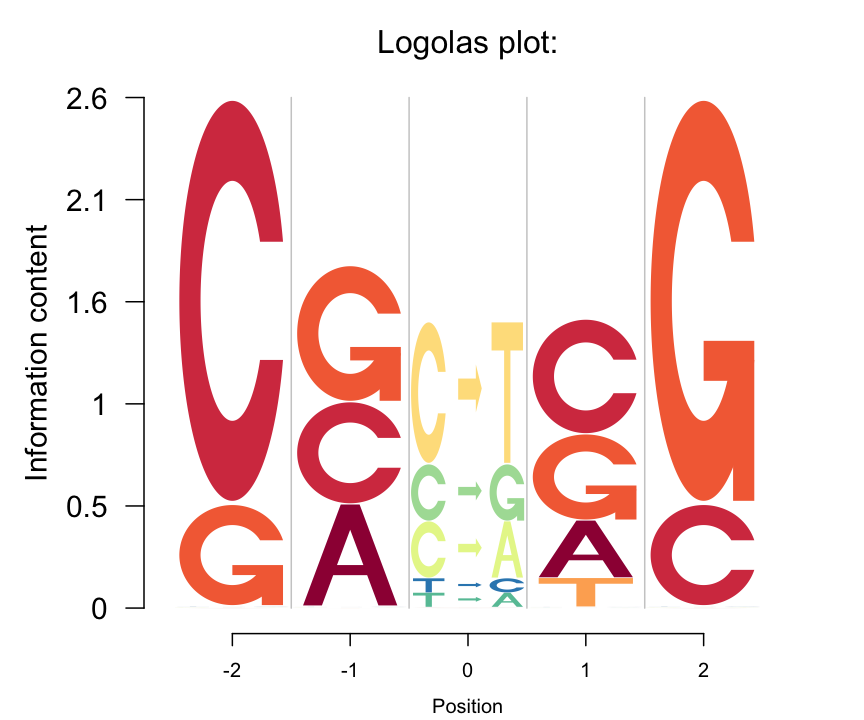
\includegraphics[width=6in,height=5in]{figure/logolas_use_7_0-1} 

\end{knitrout}
\end{center}
\end{figure}

One issue with this plot is that the user may want to have the C in \begin{verb} C>T \end{verb}
to be of the same color, but here the symbol C and \begin{verb} C>T \end{verb} are treated
as separate entities. However Logolas coloring profile provides the user the flexibility to color each symbol instead of a string. We use the color type \begin{verb} per_symbol \end{verb} instead of the \begin{verb} per_row \end{verb} profile we have been using so far.

We consider a list of all symbols \begin{verb} total_chars \end{verb} which is set as default to the list chosen above (so you can skip the \begin{verb} total_chars \end{verb} argument below). However, if the user adds a symbol to the library (the process of doing that we show in the end), then the library
is expected to grow and the user then might want to update the \begin{verb} total_chars \end{verb} list by adding new symbols.

\begin{figure}[htp]
\begin{center}
\begin{knitrout}
\definecolor{shadecolor}{rgb}{0.969, 0.969, 0.969}\color{fgcolor}\begin{kframe}
\begin{alltt}
\hlstd{cols} \hlkwb{=} \hlstd{RColorBrewer}\hlopt{::}\hlstd{brewer.pal.info[RColorBrewer}\hlopt{::}\hlstd{brewer.pal.info}\hlopt{$}\hlstd{category} \hlopt{==} \hlstr{'qual'}\hlstd{,]}
\hlstd{col_vector} \hlkwb{=} \hlkwd{unlist}\hlstd{(}\hlkwd{mapply}\hlstd{(RColorBrewer}\hlopt{::}\hlstd{brewer.pal, cols}\hlopt{$}\hlstd{maxcolors,} \hlkwd{rownames}\hlstd{(cols)))}

\hlstd{total_chars} \hlkwb{=} \hlkwd{c}\hlstd{(}\hlstr{"A"}\hlstd{,} \hlstr{"B"}\hlstd{,} \hlstr{"C"}\hlstd{,} \hlstr{"D"}\hlstd{,} \hlstr{"E"}\hlstd{,} \hlstr{"F"}\hlstd{,} \hlstr{"G"}\hlstd{,} \hlstr{"H"}\hlstd{,} \hlstr{"I"}\hlstd{,} \hlstr{"J"}\hlstd{,} \hlstr{"K"}\hlstd{,} \hlstr{"L"}\hlstd{,} \hlstr{"M"}\hlstd{,} \hlstr{"N"}\hlstd{,} \hlstr{"O"}\hlstd{,}
            \hlstr{"P"}\hlstd{,} \hlstr{"Q"}\hlstd{,} \hlstr{"R"}\hlstd{,} \hlstr{"S"}\hlstd{,} \hlstr{"T"}\hlstd{,} \hlstr{"U"}\hlstd{,} \hlstr{"V"}\hlstd{,} \hlstr{"W"}\hlstd{,} \hlstr{"X"}\hlstd{,} \hlstr{"Y"}\hlstd{,} \hlstr{"Z"}\hlstd{,} \hlstr{"zero"}\hlstd{,} \hlstr{"one"}\hlstd{,} \hlstr{"two"}\hlstd{,}
            \hlstr{"three"}\hlstd{,} \hlstr{"four"}\hlstd{,} \hlstr{"five"}\hlstd{,} \hlstr{"six"}\hlstd{,} \hlstr{"seven"}\hlstd{,} \hlstr{"eight"}\hlstd{,} \hlstr{"nine"}\hlstd{,} \hlstr{"dot"}\hlstd{,} \hlstr{"comma"}\hlstd{,}
            \hlstr{"dash"}\hlstd{,} \hlstr{"colon"}\hlstd{,} \hlstr{"semicolon"}\hlstd{,} \hlstr{"leftarrow"}\hlstd{,} \hlstr{"rightarrow"}\hlstd{)}

\hlkwd{set.seed}\hlstd{(}\hlnum{20}\hlstd{)}
\hlstd{color_profile} \hlkwb{<-} \hlkwd{list}\hlstd{(}\hlstr{"type"} \hlstd{=} \hlstr{"per_symbol"}\hlstd{,}
                      \hlstr{"col"} \hlstd{=} \hlkwd{sample}\hlstd{(col_vector,} \hlkwd{length}\hlstd{(total_chars),} \hlkwc{replace}\hlstd{=}\hlnum{FALSE}\hlstd{))}

\hlkwd{logomaker}\hlstd{(table,}
          \hlkwc{color_profile} \hlstd{= color_profile,}
          \hlkwc{total_chars} \hlstd{= total_chars,}
          \hlkwc{frame_width} \hlstd{=} \hlnum{1}\hlstd{,}
          \hlkwc{ic.scale} \hlstd{=} \hlnum{TRUE}\hlstd{,}
          \hlkwc{yscale_change}\hlstd{=}\hlnum{TRUE}\hlstd{,}
          \hlkwc{xlab} \hlstd{=} \hlstr{"Position"}\hlstd{,}
          \hlkwc{ylab} \hlstd{=} \hlstr{"Information content"}\hlstd{)}
\end{alltt}
\end{kframe}
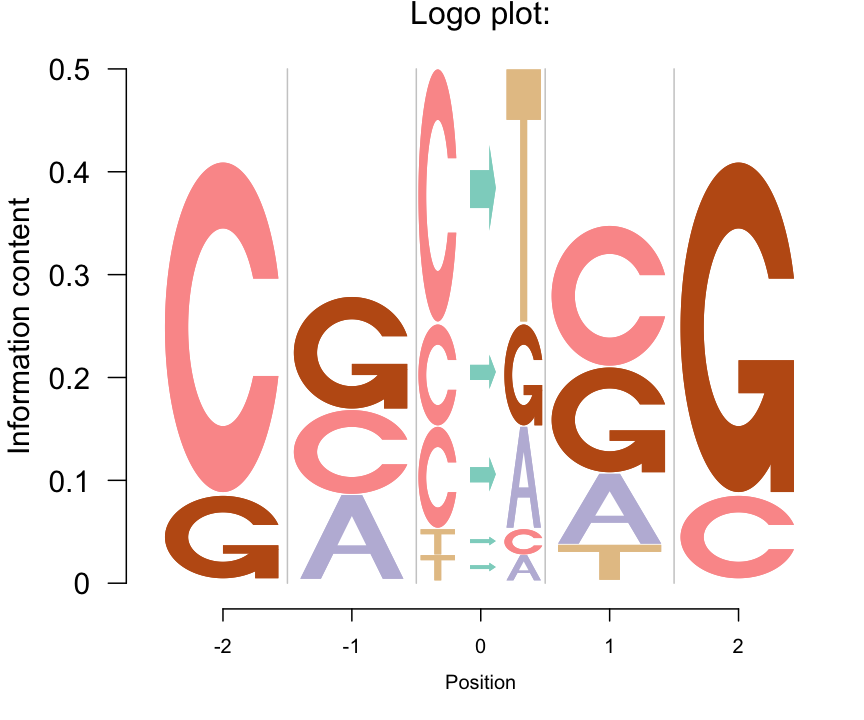
\includegraphics[width=6in,height=5in]{figure/logolas_use_7-1} 

\end{knitrout}
\end{center}
\end{figure}

Another coloring option is \begin{verb} per_column \end{verb}, in which we have a specific color for a specific column. This sort of coloring might be useful when the user wants to
highlight the difference between columns. We provide an example of this next.

\clearpage

\subsection{String Logos:  Ecological Data}

String logos can be used to represent how families or genus of species vary across sites for ecological or metagenomic data. In this case, we present an example of abundance patterns of different families of birds in three clusters of regions. The bird family names act as logos and the clusters of regions represent the stacks in the logo plot. Here the coloring pattern used is \begin{verb} per_column \end{verb} which distinguished between the different clusters of bird species.

\begin{figure}[h]
\begin{center}
\begin{knitrout}
\definecolor{shadecolor}{rgb}{0.969, 0.969, 0.969}\color{fgcolor}\begin{kframe}
\begin{alltt}
\hlkwd{set.seed}\hlstd{(}\hlnum{20}\hlstd{)}
\hlkwd{data}\hlstd{(}\hlstr{"himalayan_fauna_3_clusters"}\hlstd{)}

\hlstd{color_profile} \hlkwb{<-} \hlkwd{list}\hlstd{(}\hlstr{"type"} \hlstd{=} \hlstr{"per_column"}\hlstd{,}
                      \hlstr{"col"} \hlstd{=} \hlkwd{sample}\hlstd{(RColorBrewer}\hlopt{::}\hlkwd{brewer.pal}\hlstd{(}\hlnum{10}\hlstd{,}\hlkwc{name} \hlstd{=} \hlstr{"Spectral"}\hlstd{),}
                       \hlkwd{dim}\hlstd{(himalayan_fauna_3_clusters)[}\hlnum{2}\hlstd{],} \hlkwc{replace}\hlstd{=}\hlnum{TRUE}\hlstd{))}
\hlkwd{logomaker}\hlstd{(himalayan_fauna_3_clusters,}
          \hlkwc{color_profile} \hlstd{= color_profile,}
          \hlkwc{frame_width} \hlstd{=} \hlnum{1}\hlstd{,}
          \hlkwc{ic.scale} \hlstd{=} \hlnum{TRUE}\hlstd{,}
          \hlkwc{pop_name} \hlstd{=} \hlstr{"Bird family abundance across clusters"}\hlstd{,}
          \hlkwc{xlab} \hlstd{=} \hlstr{"Clusters"}\hlstd{,}
          \hlkwc{ylab} \hlstd{=} \hlstr{"Information content"}\hlstd{)}
\end{alltt}
\end{kframe}
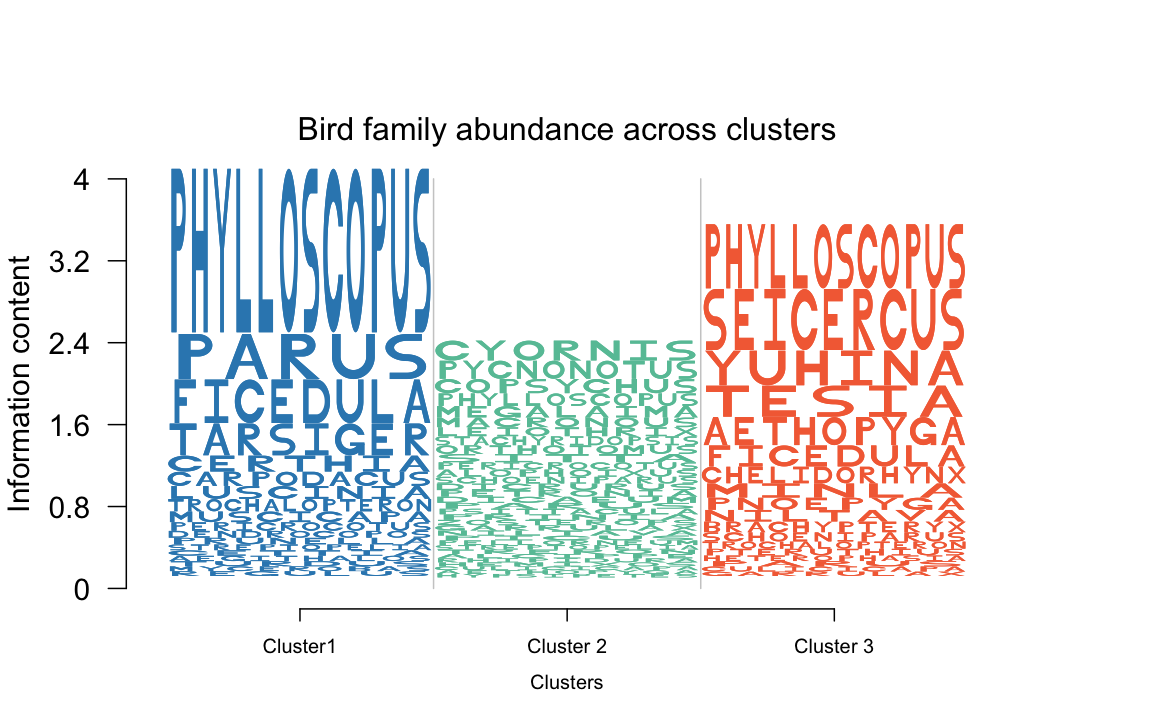
\includegraphics[width=8in,height=5in]{figure/logolas_use_10-1} 

\end{knitrout}
\end{center}
\end{figure}

\newpage

\subsection{String Logos:  Histone marks patterns}

In studies related to histone marks, one might be interested to see if certain histone marks are prominent than others in some cell lines or tissues or in some genomic regions. In this case, we apply \Logolas{} on an example data from Koch et al (2007) [Supp Table 2 of that paper] \cite{Koch2007}. The authors recorded number of histone modification sites identified by their algorithm which overlap with an intergenic sequence, intron, exon, gene start and gene end for the lymphoblastoid cell line, GM06990, in the ChIP-CHIP data. Logolas provides a handy visualization to see how the patterns of histone modification sites changes across genomic region types for that cell line.

First we input the data from Supp Table 2 due to Koch et al (2007).

\begin{knitrout}
\definecolor{shadecolor}{rgb}{0.969, 0.969, 0.969}\color{fgcolor}\begin{kframe}
\begin{alltt}
\hlstd{mat} \hlkwb{<-} \hlkwd{rbind}\hlstd{(}\hlkwd{c}\hlstd{(}\hlnum{326}\hlstd{,} \hlnum{296}\hlstd{,} \hlnum{81}\hlstd{,} \hlnum{245}\hlstd{,} \hlnum{71}\hlstd{),}
             \hlkwd{c}\hlstd{(}\hlnum{258}\hlstd{,} \hlnum{228}\hlstd{,} \hlnum{55}\hlstd{,} \hlnum{273}\hlstd{,} \hlnum{90}\hlstd{),}
             \hlkwd{c}\hlstd{(}\hlnum{145}\hlstd{,} \hlnum{121}\hlstd{,} \hlnum{29}\hlstd{,} \hlnum{253}\hlstd{,} \hlnum{85}\hlstd{),}
             \hlkwd{c}\hlstd{(}\hlnum{60}\hlstd{,} \hlnum{52}\hlstd{,} \hlnum{23}\hlstd{,} \hlnum{180}\hlstd{,} \hlnum{53}\hlstd{),}
             \hlkwd{c}\hlstd{(}\hlnum{150}\hlstd{,} \hlnum{191}\hlstd{,} \hlnum{63}\hlstd{,} \hlnum{178}\hlstd{,} \hlnum{63}\hlstd{))}

\hlkwd{rownames}\hlstd{(mat)} \hlkwb{<-} \hlkwd{c}\hlstd{(}\hlstr{"H3K4ME1"}\hlstd{,} \hlstr{"H3K4ME2"}\hlstd{,} \hlstr{"H3K4ME3"}\hlstd{,} \hlstr{"H3AC"}\hlstd{,} \hlstr{"H4AC"}\hlstd{)}
\hlkwd{colnames}\hlstd{(mat)} \hlkwb{<-} \hlkwd{c}\hlstd{(}\hlstr{"Intergenic"}\hlstd{,}\hlstr{"Intron"}\hlstd{,}\hlstr{"Exon \textbackslash{}n 1000 KB window"}\hlstd{,}
                   \hlstr{"Gene start \textbackslash{}n 1000 KB window"}\hlstd{,}\hlstr{"Gene end \textbackslash{}n 1000 KB window"}\hlstd{)}
\end{alltt}
\end{kframe}
\end{knitrout}

Note here that the histone mark symbols are alphanumeric, for example $H3K4ME1$.
We now apply \Logolas{} on this data.

\begin{figure}[h]
\begin{center}
\begin{knitrout}
\definecolor{shadecolor}{rgb}{0.969, 0.969, 0.969}\color{fgcolor}\begin{kframe}
\begin{alltt}
\hlstd{color_profile} \hlkwb{<-} \hlkwd{list}\hlstd{(}\hlstr{"type"} \hlstd{=} \hlstr{"per_row"}\hlstd{,}
                      \hlstr{"col"} \hlstd{=} \hlkwd{sample}\hlstd{(RColorBrewer}\hlopt{::}\hlkwd{brewer.pal}\hlstd{(}\hlnum{10}\hlstd{,}\hlkwc{name} \hlstd{=} \hlstr{"Spectral"}\hlstd{),}
                          \hlkwd{dim}\hlstd{(mat)[}\hlnum{1}\hlstd{]))}


\hlkwd{logomaker}\hlstd{(mat,}
          \hlkwc{color_profile} \hlstd{= color_profile,}
          \hlkwc{frame_width} \hlstd{=} \hlnum{1}\hlstd{,}
          \hlkwc{ic.scale} \hlstd{=} \hlnum{TRUE}\hlstd{,}
          \hlkwc{pop_name} \hlstd{=} \hlstr{"Histone marks in various genomic regions"}\hlstd{,}
          \hlkwc{xlab} \hlstd{=} \hlstr{""}\hlstd{,}
          \hlkwc{ylab} \hlstd{=} \hlstr{"Information content"}\hlstd{,}
          \hlkwc{yscale_change} \hlstd{=} \hlnum{TRUE}\hlstd{,}
          \hlkwc{col_line_split} \hlstd{=} \hlstr{"black"}\hlstd{)}
\end{alltt}
\end{kframe}
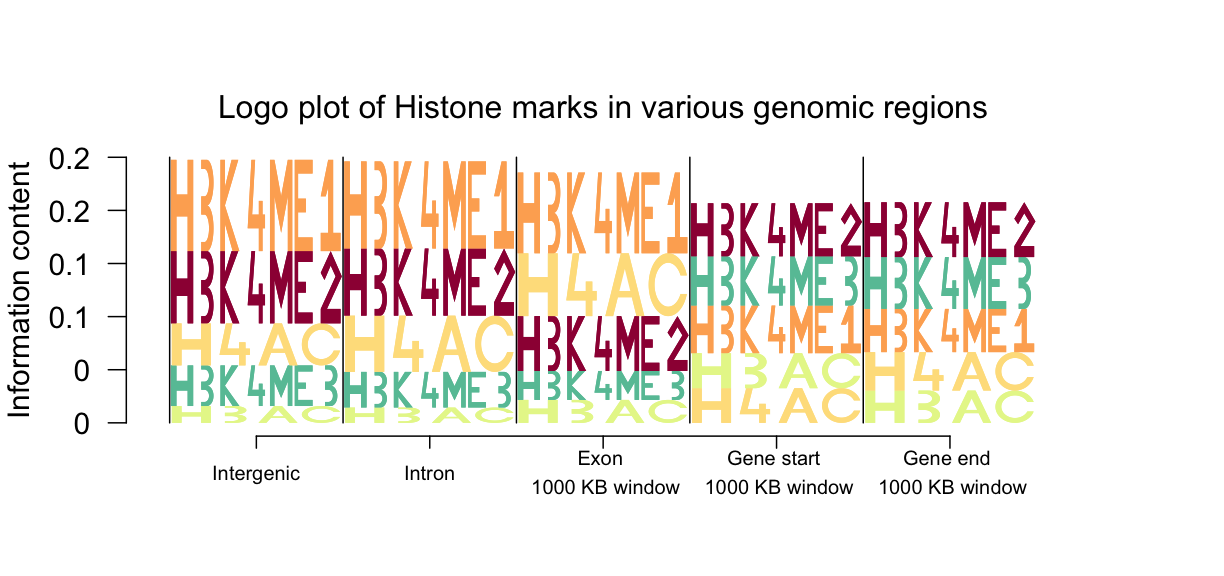
\includegraphics[width=6.5in,height=4in]{figure/logolas_use_9-1} 

\end{knitrout}
\end{center}
\end{figure}

\newpage

\subsection{String Logos:  Document mining}

So far we mainly focused on biology examples where \Logolas{} can be applied. But,
it has applications beyond the field of biology. One example application of \Logolas{} is in document mining and representing keywords or tags as logos.

Here we build a logo plot of the field categories of manuscipts submitted on aRxiv by 4 professors from Dept. of Statistics, University of Chicago. Note that the field categories here are a combination of numbers, alphabets, dots and dashes.

We first generate the data

\begin{knitrout}
\definecolor{shadecolor}{rgb}{0.969, 0.969, 0.969}\color{fgcolor}\begin{kframe}
\begin{alltt}
\hlstd{rec1} \hlkwb{<-} \hlstd{aRxiv}\hlopt{::}\hlkwd{arxiv_search}\hlstd{(}\hlstr{'au:"Matthew Stephens"'}\hlstd{,} \hlkwc{limit}\hlstd{=}\hlnum{50}\hlstd{)}
\hlstd{rec2} \hlkwb{<-} \hlstd{aRxiv}\hlopt{::}\hlkwd{arxiv_search}\hlstd{(}\hlstr{'au:"John Lafferty"'}\hlstd{,} \hlkwc{limit}\hlstd{=}\hlnum{50}\hlstd{)}
\hlstd{rec3} \hlkwb{<-} \hlstd{aRxiv}\hlopt{::}\hlkwd{arxiv_search}\hlstd{(}\hlstr{'au:"Wei Biao Wu"'}\hlstd{,} \hlkwc{limit}\hlstd{=}\hlnum{50}\hlstd{)}
\hlstd{rec4} \hlkwb{<-} \hlstd{aRxiv}\hlopt{::}\hlkwd{arxiv_search}\hlstd{(}\hlstr{'au:"Peter Mccullagh"'}\hlstd{,} \hlkwc{limit}\hlstd{=}\hlnum{50}\hlstd{)}

\hlstd{primary_categories_1} \hlkwb{<-} \hlkwd{toupper}\hlstd{(rec1}\hlopt{$}\hlstd{primary_category)}
\hlstd{primary_categories_2} \hlkwb{<-} \hlkwd{toupper}\hlstd{(rec2}\hlopt{$}\hlstd{primary_category)}
\hlstd{primary_categories_3} \hlkwb{<-} \hlkwd{toupper}\hlstd{(rec3}\hlopt{$}\hlstd{primary_category)}
\hlstd{primary_categories_4} \hlkwb{<-} \hlkwd{toupper}\hlstd{(rec4}\hlopt{$}\hlstd{primary_category)}

\hlstd{factor_levels} \hlkwb{<-} \hlkwd{unique}\hlstd{(}\hlkwd{c}\hlstd{(}\hlkwd{unique}\hlstd{(primary_categories_1),}
                   \hlkwd{unique}\hlstd{(primary_categories_2),}
                   \hlkwd{unique}\hlstd{(primary_categories_3),}
                   \hlkwd{unique}\hlstd{(primary_categories_4)))}

\hlstd{primary_categories_1} \hlkwb{<-} \hlkwd{factor}\hlstd{(primary_categories_1,} \hlkwc{levels}\hlstd{=factor_levels)}
\hlstd{primary_categories_2} \hlkwb{<-} \hlkwd{factor}\hlstd{(primary_categories_2,} \hlkwc{levels}\hlstd{=factor_levels)}
\hlstd{primary_categories_3} \hlkwb{<-} \hlkwd{factor}\hlstd{(primary_categories_3,} \hlkwc{levels}\hlstd{=factor_levels)}
\hlstd{primary_categories_4} \hlkwb{<-} \hlkwd{factor}\hlstd{(primary_categories_4,} \hlkwc{levels}\hlstd{=factor_levels)}


\hlstd{tab_data} \hlkwb{<-} \hlkwd{cbind}\hlstd{(}\hlkwd{table}\hlstd{(primary_categories_1),}
                  \hlkwd{table}\hlstd{(primary_categories_2),}
                  \hlkwd{table}\hlstd{(primary_categories_3),}
                  \hlkwd{table}\hlstd{(primary_categories_4))}

\hlkwd{colnames}\hlstd{(tab_data)} \hlkwb{<-} \hlkwd{c}\hlstd{(}\hlstr{"Matthew Stephens"}\hlstd{,}
                        \hlstr{"John Lafferty"}\hlstd{,}
                        \hlstr{"Wei Biao Wu"}\hlstd{,}
                        \hlstr{"Peter McCullagh"}\hlstd{)}

\hlstd{tab_data} \hlkwb{<-} \hlkwd{as.matrix}\hlstd{(tab_data)}
\end{alltt}
\end{kframe}
\end{knitrout}


Next, we apply \Logolas{} on the data

\begin{knitrout}
\definecolor{shadecolor}{rgb}{0.969, 0.969, 0.969}\color{fgcolor}\begin{kframe}
\begin{alltt}
\hlstd{color_profile} \hlkwb{<-} \hlkwd{list}\hlstd{(}\hlstr{"type"} \hlstd{=} \hlstr{"per_row"}\hlstd{,}
                      \hlstr{"col"} \hlstd{= RColorBrewer}\hlopt{::}\hlkwd{brewer.pal}\hlstd{(}\hlkwd{dim}\hlstd{(tab_data)[}\hlnum{1}\hlstd{],}
          \hlkwc{name} \hlstd{=} \hlstr{"Spectral"}\hlstd{))}

\hlkwd{logomaker}\hlstd{(tab_data,}
          \hlkwc{color_profile} \hlstd{= color_profile,}
          \hlkwc{frame_width} \hlstd{=} \hlnum{1}\hlstd{,}
          \hlkwc{ic.scale} \hlstd{=} \hlnum{TRUE}\hlstd{,}
          \hlkwc{pop_name} \hlstd{=} \hlstr{"arXiv field categories of UChicago STAT professors"}\hlstd{,}
          \hlkwc{xlab} \hlstd{=} \hlstr{"Professors"}\hlstd{,}
          \hlkwc{ylab} \hlstd{=} \hlstr{"Information content"}\hlstd{)}
\end{alltt}
\end{kframe}
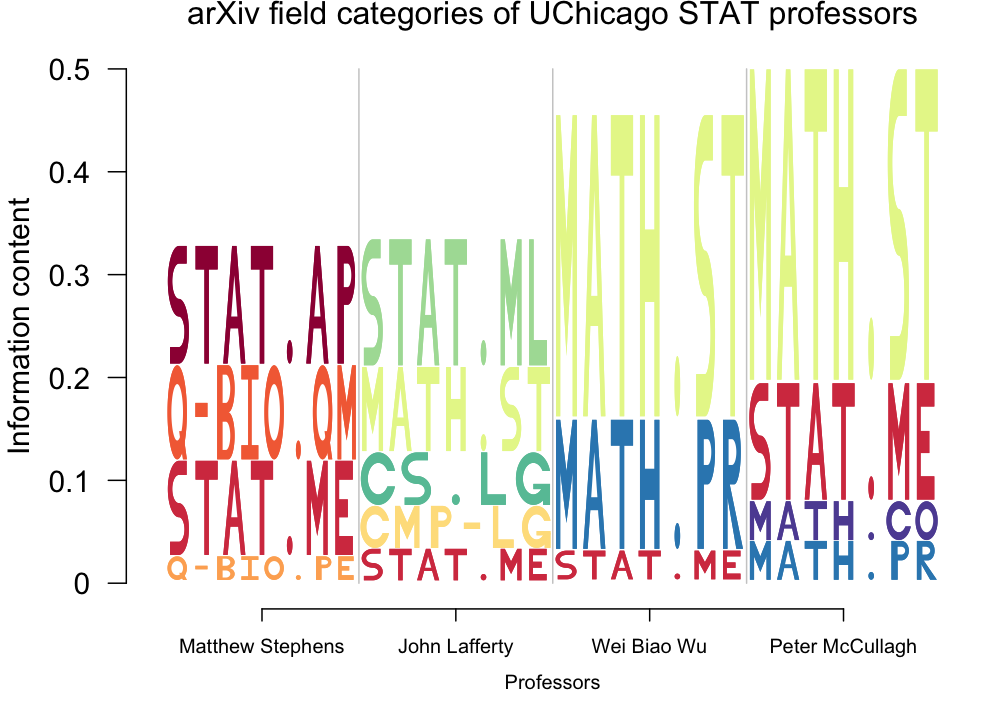
\includegraphics[width=7in,height=5in]{figure/logolas_use_12-1} 

\end{knitrout}


\section{Creating logos and adding to Library}

An user can create her own logo and add to her personalized library and \Logolas{} provides a very simple interface for doing so.

For example, if one wants to have the symbol Lambda as part of her logo,
she can create it as follows

\begin{knitrout}
\definecolor{shadecolor}{rgb}{0.969, 0.969, 0.969}\color{fgcolor}\begin{kframe}
\begin{alltt}
\hlstd{LAMBDAletter} \hlkwb{<-} \hlkwa{function}\hlstd{(}\hlkwc{colfill}\hlstd{=}\hlstr{"green"}\hlstd{)\{}

  \hlstd{x} \hlkwb{<-} \hlkwd{c}\hlstd{(}\hlnum{0.15}\hlstd{,} \hlnum{0.5}\hlstd{,} \hlnum{0.85}\hlstd{,} \hlnum{0.75}\hlstd{,} \hlnum{0.5}\hlstd{,} \hlnum{0.25}\hlstd{)}
  \hlstd{y} \hlkwb{<-} \hlkwd{c}\hlstd{(}\hlnum{0}\hlstd{,} \hlnum{1}\hlstd{,} \hlnum{0}\hlstd{,} \hlnum{0}\hlstd{,} \hlnum{0.8}\hlstd{,} \hlnum{0}\hlstd{)}

  \hlstd{fill} \hlkwb{<-} \hlstd{colfill}
  \hlstd{id} \hlkwb{<-} \hlkwd{rep}\hlstd{(}\hlnum{1}\hlstd{,} \hlkwd{length}\hlstd{(x))}

  \hlstd{ll} \hlkwb{<-} \hlkwd{list}\hlstd{(}\hlstr{"x"}\hlstd{= x,}
             \hlstr{"y"}\hlstd{= y,}
             \hlstr{"id"} \hlstd{= id,}
             \hlstr{"fill"} \hlstd{= fill)}
  \hlkwd{return}\hlstd{(ll)}
\hlstd{\}}
\end{alltt}
\end{kframe}
\end{knitrout}

The function name has to be of the form `*letter"` where the user can be creative with the `"*"` part. Also the name must be in uppercase letters. The user can then check if the symbol plot looks like a lambda or not.

\begin{figure}
\begin{center}
\begin{knitrout}
\definecolor{shadecolor}{rgb}{0.969, 0.969, 0.969}\color{fgcolor}\begin{kframe}
\begin{alltt}
\hlstd{lambda} \hlkwb{<-} \hlkwd{LAMBDAletter}\hlstd{()}
\hlstd{grid}\hlopt{::}\hlkwd{grid.newpage}\hlstd{()}
\hlstd{grid}\hlopt{::}\hlkwd{pushViewport}\hlstd{(grid}\hlopt{::}\hlkwd{viewport}\hlstd{(}\hlkwc{x}\hlstd{=}\hlnum{0.5}\hlstd{,}\hlkwc{y}\hlstd{=}\hlnum{0.5}\hlstd{,}\hlkwc{width}\hlstd{=}\hlnum{1}\hlstd{,} \hlkwc{height}\hlstd{=}\hlnum{1}\hlstd{,}
                                  \hlkwc{clip}\hlstd{=}\hlnum{TRUE}\hlstd{))}
\hlstd{grid}\hlopt{::}\hlkwd{grid.polygon}\hlstd{(lambda}\hlopt{$}\hlstd{x, lambda}\hlopt{$}\hlstd{y,}
                     \hlkwc{default.unit}\hlstd{=}\hlstr{"native"}\hlstd{,}
                     \hlkwc{id}\hlstd{=lambda}\hlopt{$}\hlstd{id,}
                     \hlkwc{gp}\hlstd{=grid}\hlopt{::}\hlkwd{gpar}\hlstd{(}\hlkwc{fill}\hlstd{=lambda}\hlopt{$}\hlstd{fill,}
                                   \hlkwc{lwd}\hlstd{=}\hlnum{10}\hlstd{))}
\end{alltt}
\end{kframe}

\includegraphics[width=4in,height=4in]{figure/logolas_use_14-1} 

\end{knitrout}
\end{center}
\end{figure}

The user can then add this symbol to the library which contains alphabets, numbers,
punctuations etc already.

To use \begin{verb} lambda \end{verb} as part of a string, the user has to put \begin{verb} lambda \end{verb} inside "/.../" to make sure that the function reads it as a new symbol and not general English alphabets or numbers. We provide an example below.


\begin{knitrout}
\definecolor{shadecolor}{rgb}{0.969, 0.969, 0.969}\color{fgcolor}\begin{kframe}
\begin{alltt}
\hlstd{counts_mat} \hlkwb{<-} \hlkwd{rbind}\hlstd{(}\hlkwd{c}\hlstd{(}\hlnum{0}\hlstd{,} \hlnum{10}\hlstd{,} \hlnum{100}\hlstd{,} \hlnum{60}\hlstd{,} \hlnum{20}\hlstd{),}
                    \hlkwd{c}\hlstd{(}\hlnum{40}\hlstd{,} \hlnum{30}\hlstd{,} \hlnum{30}\hlstd{,} \hlnum{35}\hlstd{,} \hlnum{20}\hlstd{),}
                    \hlkwd{c}\hlstd{(}\hlnum{100}\hlstd{,} \hlnum{0}\hlstd{,} \hlnum{15}\hlstd{,} \hlnum{25}\hlstd{,} \hlnum{75}\hlstd{),}
                    \hlkwd{c}\hlstd{(}\hlnum{10}\hlstd{,} \hlnum{30}\hlstd{,} \hlnum{20}\hlstd{,} \hlnum{50}\hlstd{,} \hlnum{70}\hlstd{)}
\hlstd{)}

\hlkwd{colnames}\hlstd{(counts_mat)} \hlkwb{<-} \hlkwd{c}\hlstd{(}\hlstr{"Pos 1"}\hlstd{,} \hlstr{"Pos 2"}\hlstd{,} \hlstr{"Pos 3"}\hlstd{,} \hlstr{"Pos 4"}\hlstd{,} \hlstr{"Pos 5"}\hlstd{)}
\hlkwd{rownames}\hlstd{(counts_mat)} \hlkwb{<-} \hlkwd{c}\hlstd{(}\hlstr{"R/LMBD/Q"}\hlstd{,} \hlstr{"A"}\hlstd{,} \hlstr{"X"}\hlstd{,} \hlstr{"Y"}\hlstd{)}
\end{alltt}
\end{kframe}
\end{knitrout}

LAMBDA symbol is added under \begin{verb} addlogos \end{verb} and  \begin{verb} addlogos_text \end{verb} options for the \begin{verb} logomaker \end{verb} mix of symbols.

\begin{figure}[h]
\begin{center}
\begin{knitrout}
\definecolor{shadecolor}{rgb}{0.969, 0.969, 0.969}\color{fgcolor}\begin{kframe}
\begin{alltt}
\hlstd{color_profile} \hlkwb{<-} \hlkwd{list}\hlstd{(}\hlstr{"type"} \hlstd{=} \hlstr{"per_row"}\hlstd{,}
                      \hlstr{"col"} \hlstd{= RColorBrewer}\hlopt{::}\hlkwd{brewer.pal}\hlstd{(}\hlkwd{dim}\hlstd{(counts_mat)[}\hlnum{1}\hlstd{],} \hlkwc{name} \hlstd{=} \hlstr{"Spectral"}\hlstd{))}

\hlkwd{logomaker}\hlstd{(counts_mat,}
          \hlkwc{color_profile} \hlstd{= color_profile,}
          \hlkwc{frame_width} \hlstd{=} \hlnum{1}\hlstd{,}
          \hlkwc{addlogos}\hlstd{=}\hlstr{"LMBD"}\hlstd{,}
          \hlkwc{addlogos_text}\hlstd{=}\hlstr{"LAMBDA"}\hlstd{)}
\end{alltt}
\end{kframe}
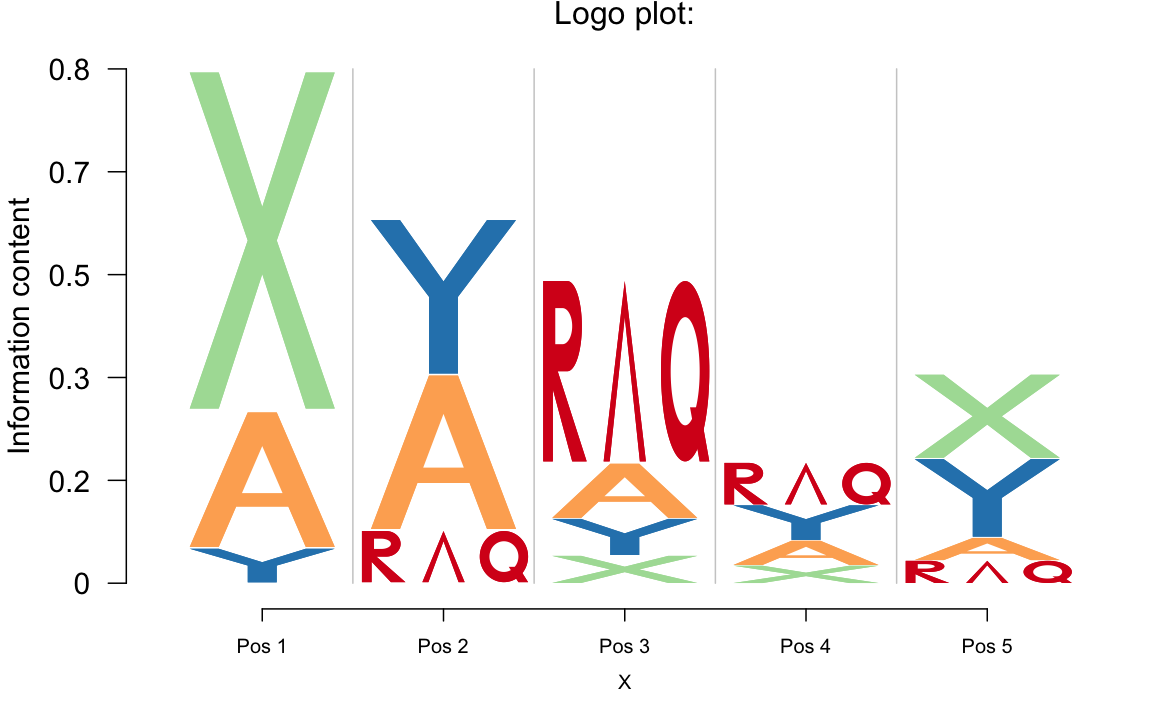
\includegraphics[width=8in,height=5in]{figure/logolas_use_17-1} 

\end{knitrout}
\end{center}
\end{figure}

\newpage

\section{Conclusion}

\Logolas{} allows an user to use alphabets, numbers, punctuations, arrows and alpha-numeric strings as logos, which expands the horizon of applicability of logo plots. Logo plots can be used as a substitute for divided bar charts and pie charts, replacing colors by actual symbols of the category represented and thereby deprecating the need for legends. It also can be used to see patterns of variation of categories (logos) observed across time points, genomic positions or any sequential variable (stacks or columns). Finally, the flexibility of creating new logos, which can be new shapes or symbols, expands the scope of logo plots even further.

\section{Acknowledgements}

We would like to acknowledge Oliver Bembom, the author of `seqLogo` for acting as an inspiration and providing the foundation on which this package is created. We would also like to thank Kevin Luo, Hussein al Asadi, John Blischak and Alex White
for helpful discussions.

\section{Session Info}

\begin{knitrout}
\definecolor{shadecolor}{rgb}{0.969, 0.969, 0.969}\color{fgcolor}\begin{kframe}
\begin{alltt}
\hlkwd{sessionInfo}\hlstd{()}
\end{alltt}
\begin{verbatim}
## R version 3.3.2 Patched (2017-01-29 r72049)
## Platform: x86_64-apple-darwin13.4.0 (64-bit)
## Running under: macOS Sierra 10.12
## 
## locale:
## [1] en_US.UTF-8/en_US.UTF-8/en_US.UTF-8/C/en_US.UTF-8/en_US.UTF-8
## 
## attached base packages:
## [1] stats     graphics  grDevices utils     datasets  methods   base     
## 
## other attached packages:
## [1] Logolas_0.99.8 knitr_1.15.1  
## 
## loaded via a namespace (and not attached):
##  [1] XML_3.98-1.5       grid_3.3.2         R6_2.2.0           stats4_3.3.2      
##  [5] magrittr_1.5       evaluate_0.10      highr_0.6          httr_1.2.1        
##  [9] stringi_1.1.2      aRxiv_0.5.10       curl_2.3           BiocStyle_2.2.1   
## [13] RColorBrewer_1.1-2 tools_3.3.2        stringr_1.1.0      seqLogo_1.40.0
\end{verbatim}
\end{kframe}
\end{knitrout}

\begin{thebibliography}{1}

\bibitem{Bembom2016}
Bembom O (2016).
\newblock seqLogo: Sequence logos for DNA sequence alignments.
\newblock R package version 1.40.0.

\bibitem{Wagih2014}
Omar Wagih (2014).
\newblock RWebLogo: plotting custom sequence logos.
\newblock R package version 1.0.3. https://CRAN.R-project.org/package=RWebLogo

\bibitem{Ou2015}
Jianhong Ou and Lihua Julie Zhu  (2015).
\newblock  motifStack: Plot stacked logos for single or multiple DNA, RNA and amino acid sequence.
\newblock  R package version 1.14.0.

\bibitem{Shiraishi2015}
Shiraishi Y, Tremmel G, Miyano S, Stephens M (2015)
\newblock A Simple Model-Based Approach to Inferring and Visualizing Cancer Mutation Signatures.
\newblock PLoS Genet 11(12): e1005657. doi: 10.1371/journal.pgen.1005657

\bibitem{Koch2007}
Koch CM, Andrews RM, Flicek P, et al (2007).
\newblock The landscape of histone modifications across $1 \%$ of the human genome in five human cell lines.
\newblock Genome Research. 2007;17(6):691-707. doi:10.1101/gr.5704207.

\end{thebibliography}

\end{document}
